\section{Assignment 6}

\subsection{Let $p_1 , p_2 , p_3$ be three points on a sphere of center $P_0$ and radius $R$. Design the trajectory such that (1) the EE will pass through the three points along the shortest path, and (2) the z axis of the EE is always orthogonal to the sphere.}

The shortest path $\gamma$ on a spherical surface lies on a great circle, which is the biggest circle that belongs to the spherical surface. Such a path is called geodesic.

First of all, the radius vectors of the starting and ending points, $p_1$ and $p_2$, of the geodesic are used to compute its direction:

\begin{equation*}
\begin{matrix}
r_1 = \frac{(p_1-p_0)}{R}\\
r_2 = \frac{(p_2-p_0)}{R}
\end{matrix}\implies r_g = r_1\cross r_2
\end{equation*}

The rotation matrix that rotates the great circle with $z=0$ to align it with the geodesic is then:

\begin{equation*}
R_\gamma = \begin{bmatrix}
r_1 & r_g\cross r_1 & r_g
\end{bmatrix}
\end{equation*}

where the cross product between $r_g$ and $r_1$ was arbitrarily chosen ($r_2$ would have worked as well) to obtain a third orthogonal direction.

Using the rotation matrix we can rotate the parametric form of the great circle as follows:

\begin{equation*}
\gamma = R_\gamma\begin{bmatrix}
R\cos(u)\\ R\sin(u)\\ 0
\end{bmatrix} + p_0
\end{equation*}

From the parametrization, we obtain the axes of the Frenet frame associated to each point:

\begin{equation*}
t = \frac{d\gamma}{du} = R_\gamma\begin{bmatrix}
-R\sin(u)\\ R\cos(u)\\ 0
\end{bmatrix}\;\;\;\;\;\;\;n = \frac{d^2\gamma}{du^2} = R_\gamma\begin{bmatrix}
-R\cos(u)\\ -R\sin(u)\\ 0
\end{bmatrix}\;\;\;\;\;\;\;b = t\cross n
\end{equation*}

The computed normal vector $n$ is always perpendicular to the sphere surface. In fact it lays on the same direction of the corresponding radius vector of the parametric geodesic:

\begin{equation*}
r_\gamma = \frac{\gamma-p_0}{R}= R_\gamma\begin{bmatrix}
\cos(u)\\ \sin(u)\\ 0
\end{bmatrix}\implies r_\gamma\cross n = R_\gamma\left(\begin{bmatrix}
\cos(u)\\ \sin(u)\\ 0
\end{bmatrix}\cross\begin{bmatrix}
-\cos(u)\\ -\sin(u)\\ 0
\end{bmatrix}\right)
\end{equation*}

The cross product in the parentheses is null for any value of $u$, therefore $n$ is always parallel to the corresponding radius vector. Since the radius vector's direction is perpendicular to the sphere by definition and the normal vector $n$ starts from a point belonging to the sphere's surface, the vector $n$ is always perpendicular to the sphere's surface.

\begin{figure}[h]
\centering
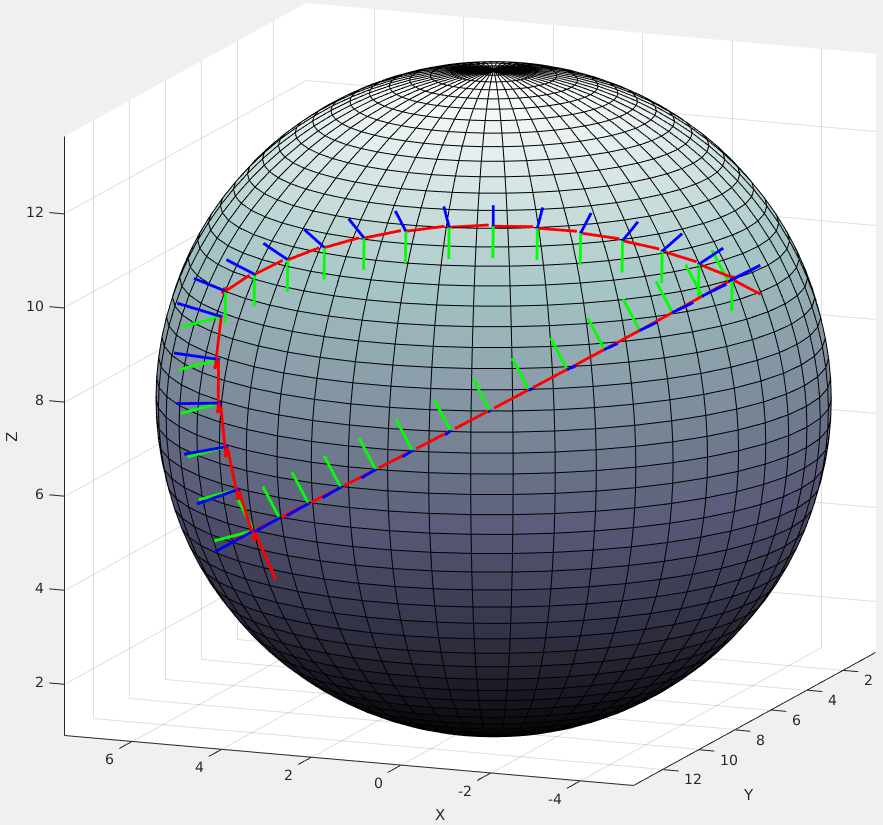
\includegraphics[keepaspectratio,width=0.8\textwidth]{sphere}
\caption{Geodesics between three random sphere points with the associated Frenet frames ($n$ in blue, $t$ in green, $b$ in red).}
\end{figure}